\documentclass[12pt]{exam}
\usepackage{amsmath}
\usepackage{amssymb}
\usepackage{amsthm}
\usepackage{tikz}
\usepackage{mathtools}
\usepackage{graphicx}
\usepackage{wrapfig}

\usepackage{bm} %bold symbols
\usepackage{hyperref} %add links

%%%%%%%%%%%%%%%%%%%%%%%%%
% 	Define vars here 	%
%%%%%%%%%%%%%%%%%%%%%%%%%

\def\hwName{Homework Set 3: §13.1 - 13.4}
\author{Zhengyu James Pan} %use like \@author
\def\email{jzpan@umich.edu}
\makeatletter

\begin{document}
%Header
\pagestyle{head}
\firstpageheader{}{}{}
\header{MATH 215}{\hwName}{\thepage}

%Solution formatting
\printanswers
\unframedsolutions

%Top matter
{\parindent0in
\begin{center}
	\bf MATH 215 FALL 2023\\
	\bf \hwName \\
	\@author\ (\href{mailto:\email}{\email})
\end{center}
}

\begin{questions}
%1
\question Do exercises 25-30 of §13.1 of \textit{Stewart’s Multivariable Calculus}.
	\\\\\textbf{Solutions:}
	\begin{questions}
		\setcounter{question}{24}
		\question \boxed{II} -- since $\sin(t)$ and $]cos(t)$ are multiplied by $t$, there is a spiral as circular arcs with increasing radius. y increases linearly.
		\question \boxed{VI} -- circles with a sudden jump in z, corresponding to the asymptote in $\frac{1}{1+t^2}$
		\question \boxed{V} -- Starts with a y-value of 1, which decreases to ~0 at larger values of t. Is a parabola when projected to x-z plane.
		\question \boxed{I} -- A circle viewed in x-y plane, z goes through two oscillations around the circle
		\question \boxed{IV} -- Circles with constant radius, increasing z according to the exponential.
		\question \boxed{III} -- Simple oscillations with linearly increasing z.
	\end{questions}
\clearpage
\setcounter{question}{1}
%2
\question Show that the space curve with parametric equation $\mathbf{r}(t) = \langle t^2 - 1, 6 + 3t - t^2, 4 - 6t\rangle$ lies in a plane, and find the equation of this plane. \textit{Hint}: If $r(t)$ lies in a plane, what must be true for $\mathbf{r'}(t)$?
	\begin{solution}
		We find the tangent vector to this curve, allowing us to search for possible normal vectors.
		\[ \mathbf{r'}(t) = \langle 2t, 3 - 2t, -6 \rangle\]
		We can see that the vector $\langle 2, 2, 1 \rangle$ will always be orthogonal with this curve, as dotting it with the tangent vector always grants 0. Thus, it lies in a plane with equation
		\[ \boxed{2(x + 1) + 2(y - 6) + (z - 4) = 0}. \tag*{\qed} \]
	\end{solution}
\clearpage

%3
\question 
	\begin{parts}
		\part Draw and parametrize the circle of radius 2 centered at $(1, 2, 0)$ and lying on the plane $x + y + z = 3$. It may help to find two orthogonal unit vectors parallel to the plane.
		\begin{solution}

			
			

			\tikzset{every picture/.style={line width=0.75pt}} %set default line width to 0.75pt        

			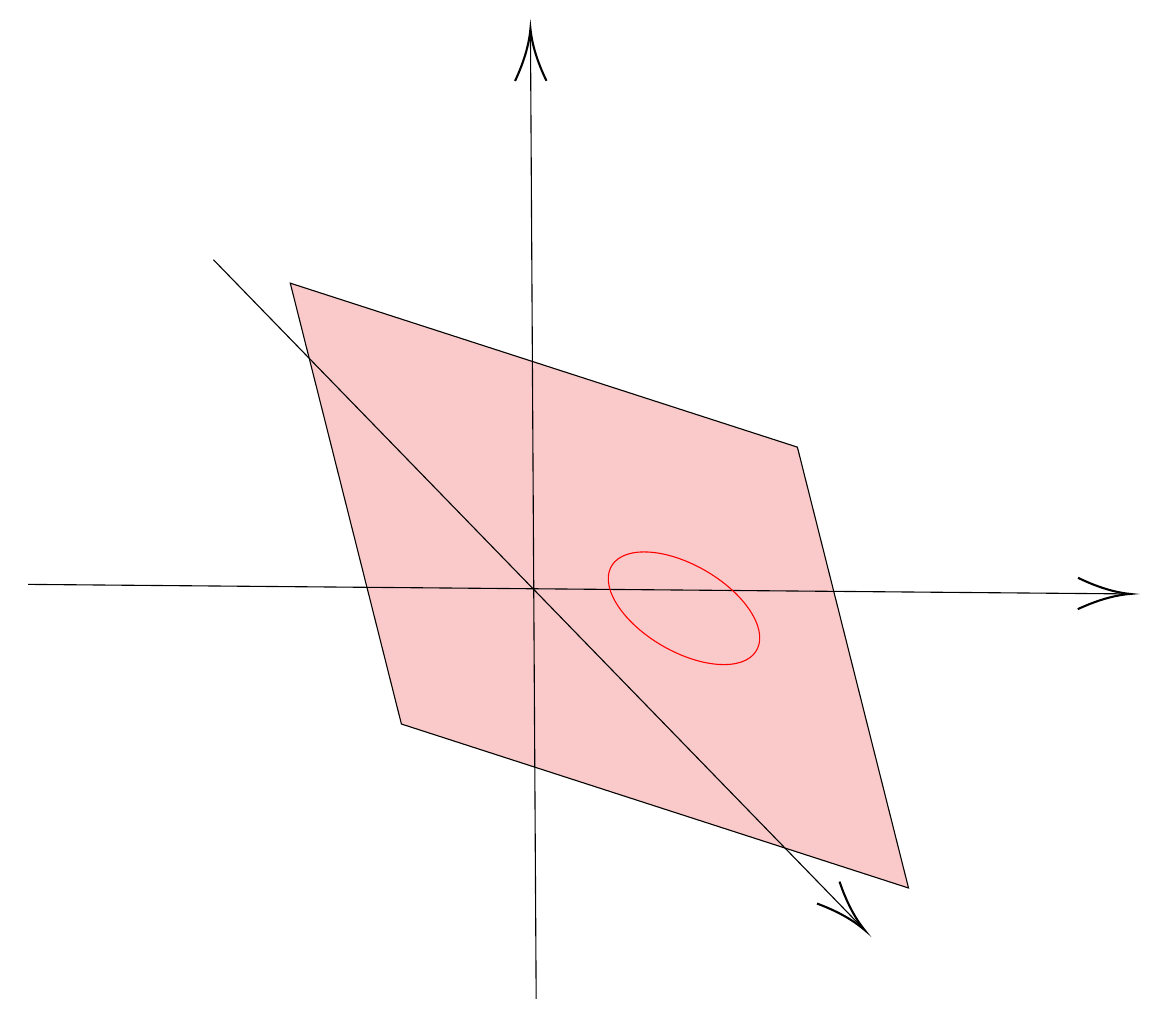
\begin{tikzpicture}[x=0.75pt,y=0.75pt,yscale=-2.3,xscale=2.3]
			%uncomment if require: \path (0,300); %set diagram left start at 0, and has height of 300

			%Shape: Parallelogram [id:dp3386268494356779] 
			\draw  [color={rgb, 255:red, 3; green, 0; blue, 0 }  ,draw opacity=1 ][fill={rgb, 255:red, 233; green, 27; blue, 27 }  ,fill opacity=0.23 ] (222.17,175.25) -- (198.89,82.9) -- (305.12,117.25) -- (328.4,209.6) -- cycle ;
			%Straight Lines [id:da5976315612243159] 
			\draw    (182.8,78) -- (317.81,216.97) ;
			\draw [shift={(319.2,218.4)}, rotate = 225.83] [color={rgb, 255:red, 0; green, 0; blue, 0 }  ][line width=0.75]    (10.93,-3.29) .. controls (6.95,-1.4) and (3.31,-0.3) .. (0,0) .. controls (3.31,0.3) and (6.95,1.4) .. (10.93,3.29)   ;
			%Straight Lines [id:da8891236273278385] 
			\draw    (250.4,232.8) -- (249.21,31.6) ;
			\draw [shift={(249.2,29.6)}, rotate = 89.66] [color={rgb, 255:red, 0; green, 0; blue, 0 }  ][line width=0.75]    (10.93,-3.29) .. controls (6.95,-1.4) and (3.31,-0.3) .. (0,0) .. controls (3.31,0.3) and (6.95,1.4) .. (10.93,3.29)   ;
			%Straight Lines [id:da4262954076409089] 
			\draw    (144,146) -- (372.8,147.98) ;
			\draw [shift={(374.8,148)}, rotate = 180.5] [color={rgb, 255:red, 0; green, 0; blue, 0 }  ][line width=0.75]    (10.93,-3.29) .. controls (6.95,-1.4) and (3.31,-0.3) .. (0,0) .. controls (3.31,0.3) and (6.95,1.4) .. (10.93,3.29)   ;
			%Shape: Ellipse [id:dp8850500969361768] 
			\draw  [color={rgb, 255:red, 255; green, 0; blue, 0 }  ,draw opacity=1 ] (267.87,151) .. controls (263.27,144.48) and (265.57,139.2) .. (273.03,139.2) .. controls (280.48,139.2) and (290.25,144.48) .. (294.86,151) .. controls (299.47,157.52) and (297.16,162.8) .. (289.71,162.8) .. controls (282.25,162.8) and (272.48,157.52) .. (267.87,151) -- cycle ;

			\end{tikzpicture}

			A parallel orthogal unit vector to this plane is $\langle 0, \frac{1}{\sqrt{2}}, -\frac{1}{\sqrt{2}} \rangle$. Finding the cross product and normalizing, we get $\langle -\frac{2}{\sqrt{6}}, \frac{1}{\sqrt{6}}, \frac{1}{\sqrt{6}} \rangle$ We can treat this as a basis for 2D coordinates on the given plane. Multiplying $2\sin(t)$ by the first and $2\cos(t)$ by the second respectively will give the parameterized terms. Then the total parametric equation of the circle is 
			\[ \boxed{\langle 1 - \frac{4}{\sqrt{6}}\cos(t), 2 + \sqrt{2}\sin(t) + \frac{2}{\sqrt{6}}\cos(t), 0 - \sqrt{2}\sin(t) + \frac{2}{\sqrt{6}}\cos(t) \rangle} \tag*{\qed} \]
			
		\end{solution}
	\end{parts}
		\clearpage
		\setcounter{question}{2}
		\question \begin{parts} 
			\setcounter{partno}{1}
			\part Find parametric equations for two circles $C_1$ and $C_2$ in space such that 
			\begin{itemize}
				\item $C_1$ and $C_2$ have the same radius
				\item $C_1$ and $C_2$ intersect at the points (0, 1, 0) and (0, 0, 1) and nowhere else.
			\end{itemize}
			\begin{solution}
				We can create circles centered at (0, 0, 0) and (0, 1, 1) with radius 1. The equations for these would be 
				\begin{center}
					\[ \boxed {C_1 = \langle 0, \sin(t), \cos(t)} \] \\
					and
					\[\boxed{C_2 = \langle 0, 1 + \sin(t), 1 + \cos(t)} \tag*{\qed} \]
				\end{center}
			\end{solution}
		\end{parts}
\clearpage
%4 
\question Consider the curves $C_1$ and $C_2$ with parametrizations given by
	\[ \mathbf{r_1}(t) = \left\langle t, 2t^2, - \frac{1}{t} \right\rangle \text{ and } \mathbf{r_2}(t)= \langle 1 - t, 2 \cos t, \sin t - 1 \rangle \]
	\begin{parts}
		\part Show that these two curves intersect, and find the point(s) of intersection.
		\begin{solution}
			For the curves to intersect, all three of $x$, $y$, and $z$ must be equal between both curves. Then 
			\begin{align*}
				\begin{cases}
					t_1 + t_2 = 1 \\
					2t_1^2 = 2\cos(t_2) \\
					-\frac{1} {t_1} = \sin(t_2)-1
				\end{cases}
			\end{align*}
			We prefer $t_1$ since it is equal to $x$.
			\begin{align*}
				\begin{cases}
					t_1^2=\cos(1 - t_1) \\
					-\frac{1} {t_1} + 1= \sin(1-t_1)
				\end{cases}
			\end{align*}
			Unfortunately, I don't know how to solve this by hand, although $t_1 = 1$ can be found easily by guess and check. This corresponds to $\boxed{(1, 0, -1)}$.\qed
		\end{solution}
		\part Find the angle of intersection between the two curves at any points of intersection (i.e. the angle between the tangent vectors).
			\begin{solution}
				This is given by the dot product of unit tangent vectors. For $C_1$:
				\[ \langle 1, 4t, \frac{1}{t^2} \rangle \div \sqrt{1+16t^2 + \frac{1}{t^4}}\]
				For $C_2$: 
				\[ \langle -1, -2\sin(t), \cos(t) \rangle \div \sqrt{1+4\sin^2(t)+\cos^2(t)} \]
				At $x=1$, this dot product is equal to 
				\[ \frac{-1 * 1 + 4 * 0 + 1 * 1 }{... \neq 0} = \frac{1 - 1}{...} = \boxed{0} \tag*{\qed}\]
			\end{solution}
	\end{parts}
\clearpage
%5
\question The plane curve with parametrization $r(t) = \langle e^t \cos 2t, e^t \sin 2t\rangle, t \in \mathbb{R}$, is an example of a Bernoulli
spiral. Show that the angle $\varphi$ between the position vector $\mathbf{r}(t)$ and the tangent vector $\mathbf{r}'(t)$ is constant, and find the value of $\varphi$ in radians to two decimal places.
	\begin{solution}
		We find the dot product of the position and tangent vector:
		\begin{align*}
			\mathbf{r} \cdot \mathbf{r'} &= \langle e^t \cos 2t, e^t \sin 2t \rangle \cdot \langle e^t \cos 2t - 2e^t \sin 2t, e^t \sin 2t + 2e^t \cos 2t \rangle \\
			&= e^{2t} \cos^2 2t - e^{2t} \cos 2t \sin 2t + e^{2t} \sin^2 2t + e^{2t} \cos 2t \sin 2t \\
			& = e^{2t} \cos^2 2t + e^{2t} \sin^2 2t \\
			&= e^{2t}
		\end{align*}
		The norms of $\mathbf{r}$ and $\mathbf{r'}$ respectively are $e^t$ and $\sqrt{5}e^t$, so the cos of the angle is thus a constant $\frac{1}{\sqrt{5}}$. Then 
		\[ \arccos (\frac{1}{\sqrt{5}}) = \boxed{\varphi = 1.107148718} \tag*{\qed} \]
	\end{solution}
\clearpage
%6
\question A wheel of radius R traces out a cycloid.
	\begin{parts}
		\part Find a parametrization, $\mathbf{c} (t)$, of this cycloid such that a single arch is traced out from $t = 0$ to $t = 2\pi$ (a single revolution of the wheel). Choose your coordinate system so that $\mathbf{c} (0)= (0, 0)$.
		\begin{solution}
			\[ \boxed{\mathbf{c} (t) = \langle R(t-\sin(t)),\ R(1-\cos(t)) \rangle} \tag*{\qed}\]
		\end{solution}
		\part Find the length of a single arch.
			\begin{solution}
				\begin{align*}
					\int_{0}^{2\pi}\sqrt{\frac{dx}{dt}^2+\frac{dy}{dt}^2}dt &= \int_{0}^{2\pi}R\sqrt{(1-\cos(t))^2+(\sin(t))^2}dt \\
					&= \int_{0}^{2\pi}R\sqrt{2 - 2\cos(t)}dt \\
					&= \boxed{8R} \tag*{\qed}
				\end{align*}
			\end{solution}
	\end{parts}
\clearpage
%7
\question An \textit{involute} is the curve traced out by the end of a taut string being unwound from a given curve, in the plane of the curve. Let's consider the circle involute that arises when we unwind string from a spool. In the figure below the unwound string is shown in purple, the angle between the green line segment and the purple line segment is $\frac{\pi}{2}$, and the spool, which has radius R, is shown in orange. The circle involute is shown in black, and we wish to parametrize the circle involute in terms of the angle $\theta$; that is, we want to find a vector valued function $\mathbf{r}(\theta)$ for $\theta \geq 0$ so that its associated space curve is the circle involute.\\
\begin{center}
	\includegraphics*[scale=0.3]{images/03-involute.png}
\end{center}
	\begin{parts} 
		\part What is the length of the unwound thread (that is, the purple line segment) as a function of $\theta$?
			\begin{solution}
				Since the thread is taut around the circumference of the circle, it the length unraveled is equal to the arclength which $\theta$ has already passed through. This is equal to $\boxed{R\theta }$.
			\end{solution}
		\part What is $\mathbf{r}(\theta)$? Hint: It may help to first find the vector that moves from the origin to the edge ofthe circle (the green line in the diagram) and then find the vector that moves from the edge of the circle to the involute (the purple line in the diagram).
			\begin{solution}
				The green vector can simply use the parametric equation of a circle with radius $R$:  $\langle R\cos(\theta), R\sin(\theta) \rangle$. \\
				The purple vector is a vector with direction perpendicular to the radius and a magnitude equal to the length of the string. The direction can be given by $\langle \sin(\theta), -\cos(\theta) \rangle$. Multiplying by the magnitude, we get $\langle R\theta\sin(\theta), -R\theta\cos(\theta) \rangle$. Adding the two together, we find $\boxed{\mathbf{r}(\theta) = \langle R\cos(\theta) + R\theta\sin (\theta), R\sin(\theta) - R\theta\cos(\theta) \rangle}$. \qed
			\end{solution}
		\clearpage
		\end{parts}
\setcounter{question}{6}
\question 
	\begin{parts}
		\setcounter{partno}{2}
		\part What is the length of the curve from $\theta = 0$ to $\theta = b$?
			\begin{solution}
				Using the arclength formula:
				
				\begin{align*}
					\int_{0}^{b} \sqrt{(\frac{dx}{d\theta})^2+ (\frac{dx}{d\theta})^2} &= \int_{0}^{b} R\sqrt{(\theta \cos(\theta) + \sin(\theta) - \sin(\theta))^2 + (\theta \sin(\theta) + \cos(\theta) - \cos(\theta))^2} d\theta \\
					&= \int_{0}^{b} R\sqrt{(\theta \cos(\theta) )^2 + (\theta \sin(\theta))^2} d\theta \\
					&= \int_{0}^{b} R\sqrt{\theta^2} d\theta \\
					&= \int_{0}^{b} R\theta d\theta \\
					&= \boxed{\frac{Rb^2}{2}} \tag*{\qed}
				\end{align*}
			\end{solution}
		\part Parametrize the circle involute in terms of arc length.
			\begin{solution}
				We found the arclength $s=\frac{R\theta^2}{2}$. The parametrization in terms of $s$ is thus
				\[ \boxed{\mathbf{r}(s) = \langle R\cos\left(\sqrt{\frac{2s}{R}}\right) + R\sqrt{\frac{2s}{R}}\sin \left(\sqrt{\frac{2s}{R}}\right), R\sin\left(\sqrt{\frac{2s}{R}}\right) - R\sqrt{\frac{2s}{R}}\cos\left(\sqrt{\frac{2s}{R}}\right) \rangle} \]
			\end{solution}
		\part Compute the curvature of the circle involute. \textit{Hint:} The book contains several different ways to compute the curvature $\kappa$. Some may be easier than others. 
			\begin{solution}
				We can compute the curvature by calculating the magnitude of the derivative of the unit tangent vector $\bm{T'}(\theta)$ and dividing by the magnitude of the tangent vector $\mathbf{r'}(\theta)$. 
				The tangent vector is 
				\begin{align*}
					\mathbf{r'}(\theta) &= \langle -R\sin(\theta) + R\sin (\theta) + R\theta\cos(\theta), R\cos(\theta) - R\cos(\theta) + R\theta\sin(\theta)\rangle \\
					&= \langle R\theta\cos(\theta), R\theta\sin(\theta) \rangle
				\end{align*}
				Of course, the unit tangent vector is then just the parametric equation of a circle. The derivative of the unit tangent vector is still a parametric circle, so it has magnitude 1. The tangent vector has magnitude $R\theta$, so the curvature of the involute is \[\boxed{\frac{1}{R\theta}} \tag*{\qed}\]
			\end{solution}
	\end{parts}
\clearpage
%8
\question A quarterback intends to throw a pass to score a touchdown. Suppose the quarterback is 20 yards from
	the endzone, and the receiver is standing $\ln (21 + \sqrt{440})$ yards to the left of the quarterback. (The
	receiver is very good at calculus, and so knows the correct position to stand at to make this work -- it is
	approximately 3.737 yards, or just over 11 feet.) The receiver will always run directly at the location of
	the ball (this is not the most efficient path to catching the ball, but it does allow for flexibility if plans
	change, i.e. a member of the opposing team intercepts the ball). Because the ball is moving, this means
	that the receiver will trace out a special curve called a catenary. For simplicity, suppose the receiver
	is placed at the origin, and the quarterback is at the point $(\ln (21 + \sqrt{440}) , 0, 0)$. To make the play
	as efficiently as possible, the quarterback wants the receiver to catch the ball as soon as they hit the
	end zone, i.e. at the point $(\ln (21 + \sqrt{440}) , 20, 0)$. In this coordinate system, the path of the receiver is given by
	\[ \mathbf{r}(x) = \langle x, \cosh(x) - 1, 0 \rangle, \]
	where we recall the definitions of the hyperbolic sine and cosine functions as given by
	\[\sinh(x) = \frac{e^x-e^{-x}}{2} \text{ and } \cosh(x) = \frac{e^x + e^{-x}}{2}\]
	\begin{parts}
		\part If the quarterback can throw the ball with a speed of 50 feet per second, at what angle above the
		ground should the quarterback throw the ball? Remember that the motion of the football is in the
		$yz$-plane in this coordinate system, and the acceleration due to gravity is given by $\langle 0, 0, -g\rangle$, with
		$g = 32 $ ft/s$^2$.
			\begin{solution}
				Let $\theta$ be the angle at which the quarterback throws the ball. Then the ball's path by time can be parameterized as 
				\[ \left\langle \ln (21 + \sqrt{440}) , 50\cos(\theta)t, -\frac{g}{2}t^2+50\sin(\theta)t \right\rangle.\]
				We know that at time $t_f$ when the ball lands/is caught, the z-coordinate is 0. So, $t_f=\frac{100\sin(\theta)}{g}$. Utilizing the additional fact that the y-coordinate will be 20 at $t_f$, we find that 
				\begin{align*}
					\frac{5000\sin\cos(\theta)}{g} &= 20 \\
					\frac{2500\sin(2\theta)}{g} &= 20 \\
					\theta &= \frac{\arcsin\left(\frac{20g}{2500}\right)}{2} \\
					\theta &= \boxed{0.1294410168 \text{ rad} = 7.41642396^\circ} \tag*{\qed}
				\end{align*}
			\end{solution}
		\clearpage
		\end{parts}
\setcounter{question}{7}
\question 
	\begin{parts}
		\setcounter{partno}{1}
		\part How fast does the receiver need to run in order to catch the ball?
			\begin{solution}
				Taking derivatives with respect to $x$, the total arclength of the receiver's path is 
				\begin{align*}
					\int_{0}^{\ln (21 + \sqrt{440})} \sqrt{1 + (-\sinh(x))^2}dx &= \int_{0}^{\ln (21 + \sqrt{440})} \sqrt{1+\frac{(e^x-e^{-x})^2}{4}}dx \\
					&= \int_{0}^{\ln (21 + \sqrt{440})} \sqrt{1+\frac{e^2x+2+e^{-2x}}{4}}dx \\
					&= \int_{0}^{\ln (21 + \sqrt{440})} \sqrt{\cosh^2(x)}dx \\
					&= \int_{0}^{\ln (21 + \sqrt{440})} \cosh(x)dx \\
					&= \sinh(\ln (21 + \sqrt{440})) - 0 \\\\
					&= \frac{21+\sqrt{440} - \frac{1}{21+\sqrt{440}}}{2} \\
					&= 2\sqrt{110}
				\end{align*}
				This is the distance the receiver needs to run within time $t_f$. Thus the speed he needs to run is $\frac{2\sqrt{110}}{0.40337455} = \boxed{52.00173626 \text{ft/s}}$. \qed
			\end{solution}
	\end{parts}
\clearpage
%9
\question The Fresnel cosine integral, C, and the Fresnel sine integral, S are defined by
	\[C(x) = \int_{0}^{x}\cos(u^2)du\text{ and } S(x) = \int_{0}^{x}\sin(u^2)du. \]
	The Cornu spiral is the space curve parametrized by the vector valued function $\mathbf{r}(t) = \langle S(t), C(t)\rangle$ for $t\in \mathbb{R}$.
	\begin{parts}
		\part Show that $\mathbf{r}(t)$ parametrizes the Cornu spiral by arc length.
		\begin{solution}
			The arclength of the Cornu spiral from $t=0$ to $t=s$ using this parameterization is 
			\begin{align*}
				\int_{0}^{s} \sqrt{\left(\frac{dx}{d\theta}\right)^2+ \left(\frac{dx}{d\theta}\right)^2} &= \int_{0}^{s} \sqrt{\cos^2(t^2)+\sin^2(t^2)}dt \\
				&= \int_{0}^{s} \sqrt{1}dt \\
				&= \int_{0}^{s} 1 dt \\
				&= s
			\end{align*}
			Therefore the arclength from $\mathbf{r}(0)$ to $\mathbf{r}(t)$ is simply $t$. \qed
		\end{solution}
		\part Show that, for $t \geq 0$, the curvature of a Cornu spiral is a linear function of arc length. Hint: The book contains several different ways to compute the curvature $\kappa$. Some may be easier than others.
		\begin{solution}
			The curvature is equal to $\left|\frac{dT}{ds}\right|$, equivalently $\left|\frac{\frac{dT}{dt}}{\frac{ds}{dt}}\right|$. Since we established that $s=t$, it follows that $\frac{ds}{dt} = 1$.
			So, we simply find derivative of the tangential vector.
			\begin{align*}
				T &= \frac{\mathbf{r}'(t)}{ \left|\mathbf{r}'(t)\right| } \\
				&= \langle \cos(t^2), \sin(t^2) \rangle \div \sqrt{\cos^2(t^2)+\sin^2(t^2)}\\
				&= \langle \cos(t^2), \sin(t^2) \rangle \div 1 \\
				&= \langle \cos(t^2), \sin(t^2) \rangle \\
				T' &= \langle - 2t\sin(t^2), 2t\cos(t^2) \rangle
			\end{align*}
			Then, the norm of $T'$ is 
			\begin{align*}
				\sqrt{4t^2\sin^2(t^2) + 4t^2\cos^2(t^2)} &= \sqrt{4t^2} \\
				&= \boxed{2t} \tag*{\qed}
			\end{align*}
		\end{solution}
		\part Cornu spirals are used when designing highway exit ramps. Offer an explanation for why they might be used in such a way. 
		\begin{solution}
			Since Cornu spirals have linearly increasing curvature, it provides a very even transition for cars driving along the ramp, without any sudden changes in curvature which could cause dangerous bumps. \qed
		\end{solution}
	\end{parts}
\end{questions}

\end{document}